\documentclass{article}
\usepackage[a4paper, tmargin=1in, bmargin=1in]{geometry}
\usepackage[utf8]{inputenc}
\usepackage{graphicx}
\usepackage[justification=centering]{caption}

% \usepackage{parskip}
\usepackage{pdflscape}
\usepackage{listings}
\usepackage{hyperref}
\usepackage{caption}
\usepackage{subcaption}
\usepackage{float}
\usepackage{amsmath}
\DeclareMathOperator*{\argmax}{\arg\!\max}
\title{CS 747 : Foundations of Intelligent Learning Agents Assignment 3}
\author{Arka Sadhu - 140070011}
\date{\today}

\begin{document}
\maketitle

\section{Q-learning}
For q-learning the following has been done:
\begin{itemize}
\item We continue a particular episode until a terminal state is reached, or the number of iterations for the particular episode has crossed a certain threshold, in this case 1000. The learning rate is set to 0.5
\item When the agent is initialized, a q-table for each corresponding state and action is initialized. Here we initialize it with all 0's. A learning rate is suitably chosen.
\item The first action is given as random. The reward, next state and event is received from the server. If the goal is reached, the reward is 100, anything else is awarded a reward of -1. The event is either continue, terminated or goal reached.
\item We note the events. If it is either terminated or goal reached we update the corresponding q-table and then start a new episode. If it is continued we only udpate the q-table.
\item The update of q-table includes two steps. First the action which gives the highest q-value in the next state is chosen. This is then used to update the value in the q-table corresponding to current state and current action.
  $$Q[s, a] = Q[s, a] + \alpha * (reward +  \gamma * \max_a Q(s', a) - Q(s, a))$$
\item When asked for the next action, the agent chooses the action in an epsilon greedy manner from the q-table values corresponding to the current state. The epsilon is decayed in $\frac{1}{n}$ manner where n is the episode number.
\item For plotting the graphs, we have used 50 random seeds for each instance 0 and 1, and then taken the average reward for each episode.
\end{itemize}

% \begin{figure}[H]
%   \centering
%   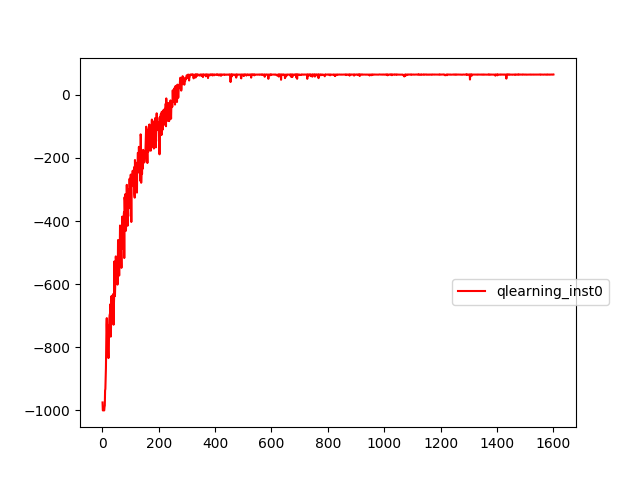
\includegraphics[scale=0.5]{images/qlearn_instance_0}
%   \caption{Q-learning for instance 0}
%   \label{fig:ql0}
% \end{figure}

% \begin{figure}[H]
%   \centering
%   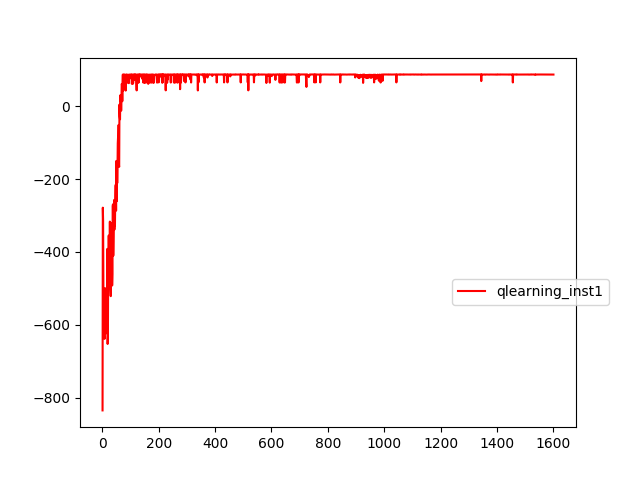
\includegraphics[scale=0.5]{images/qlearn_instance_1}
%   \caption{Q-learning for instance 1}
%   \label{fig:ql1}
% \end{figure}

% \begin{figure}[H]
%   \centering
%   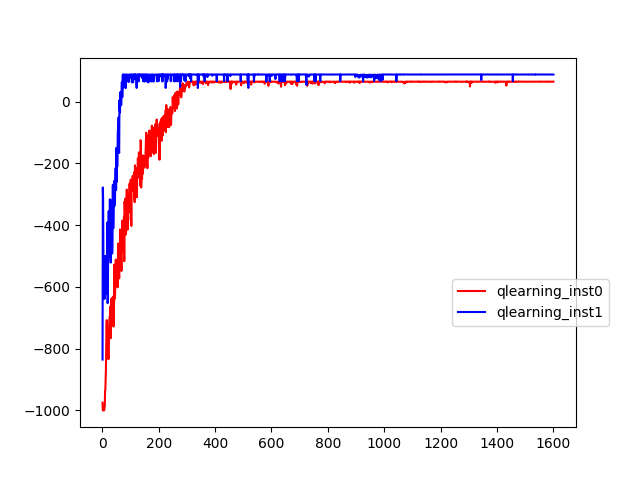
\includegraphics[scale=0.5]{images/qlearn_instance_0_1}
%   \caption{Q-learning both instance 0 and 1}
%   \label{fig:ql01}
% \end{figure}
\section{Sarsa ($\lambda$)}
For sarsa ($\lambda$) the following has been done:
\begin{itemize}
\item All the initializations are the same as in Q-learning. The only difference is that we initialize a new matrix called the eligibility matrix of the same size of the q-table to all zeros. Also we choose the first action at random.
\item The same steps are followed as in Q-learning when the reward, next state and the event is given. As an extra we re-initialize the eligibility trace to all zeros when the episode either terminates or goal is reached. Next we update the q-table and the eligibility trace.
\item Now given the new state, we choose a new action using some epsilon greedy method on the q-table. Here this strategy is kept the same as that followed for q-table. We call this action as a'.
\item We use this a' for computing the update. First we initialize another variable $\delta$ which is computed as :
  $$\delta = reward + \gamma * Q(s', a') - Q(s, a)$$
\item Next depending on the trace strategy we update the eligibility trace corresponding to the current state and action. If accumulative trace is used then we add 1 to the existing value. If replacing trace is used we re-assign the existing value to 1.
\item Then for all states and all actions (basically the whole matrix) we do the following udpates:
  $$Q = Q + \alpha * \delta * eligibility\_trace$$
  $$eligibility\_trace = \gamma * \lambda * eligibility\_trace$$
\item For the next action we choose a'.
\item Again for the plots we have averaged over 50 random seeds for each episode.
\end{itemize}

\subsection{Selecting the best Lambda}
There could be two metrics  which can be used to decide the best lambda
\begin{itemize}
\item The lambda which converges faster and gives a reasonable sub-optimal value.
\item The lambda which gives a higher optimal value.
\end{itemize}
From the experiments it is found that for smaller lambda the algorithm converges slower but the value to which it converges is higher. On the other hand a larger lambda results in the algorithm to converge much faster but the value to which it converges is sub-optimal that is it is lower.

The two metrics can be thought of as follows. If I want the agent to learn the optimal path irrespective of the number of episodes it takes then the second metric should be considered. If on the other hand we want the total cumulative reward across the episodes to be higher in a finite time then we can go for the first option.

% Here if the second metric is considered. As a result $\lambda=0$ is chosen to be the optimal lambda and the plots are as shown below.
\begin{figure}[H]
  \centering
  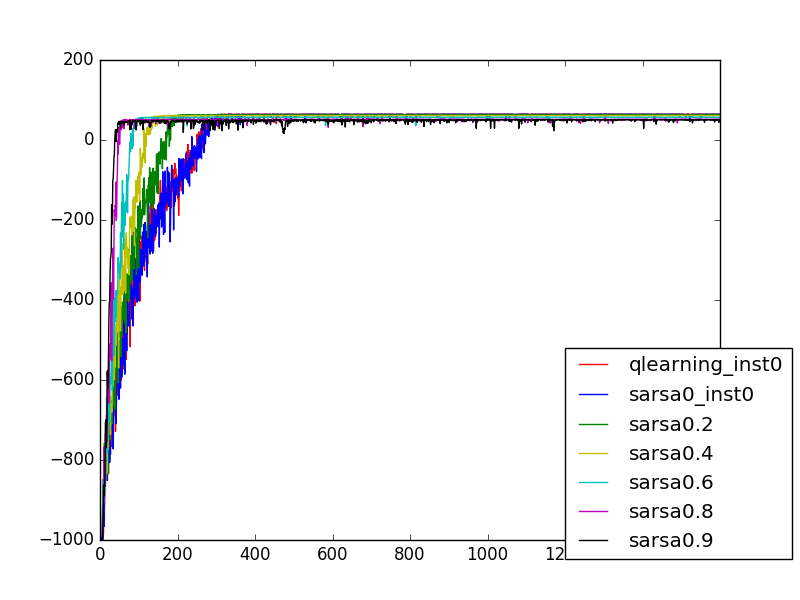
\includegraphics[scale=0.5]{images/all_instance_0}
  \caption{All plots together Instance 0}
  \label{fig:allinst0}
\end{figure}

\begin{figure}[H]
  \centering
  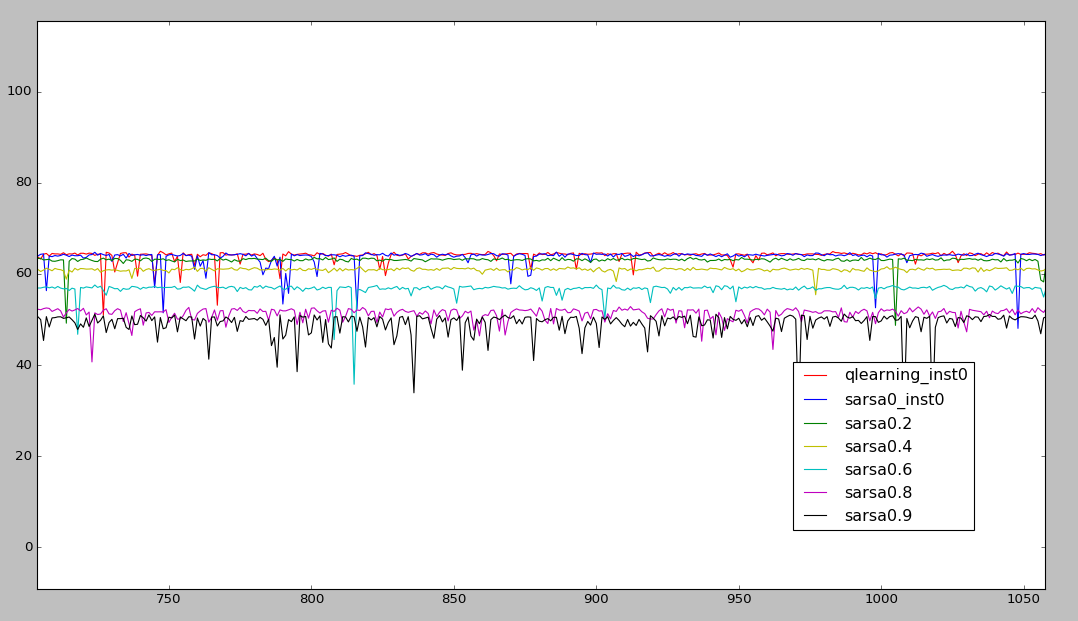
\includegraphics[scale=0.25]{images/all_plots_inst0_converg}
  \caption{All plots together at convergence Instance 0}
  \label{fig:allinst0conv}
\end{figure}

If the second metric is considered then $\lambda=0$ should be chosen since it achieves the optimal value, if instead the first metric is considered $\lambda=0.9$ should be considered. Results with both are shown in the plots.

\section{Plotting Q-learning and Sarsa ($\lambda$)}
The y-axis is the expected cumulative reward against x-axis which is episode number. Here the expectation is over the 50 random seeds.

\subsection{Plots for Instance 0 and 1 for Q-learning and Sarsa 0}

\begin{figure}[H]
  \centering
  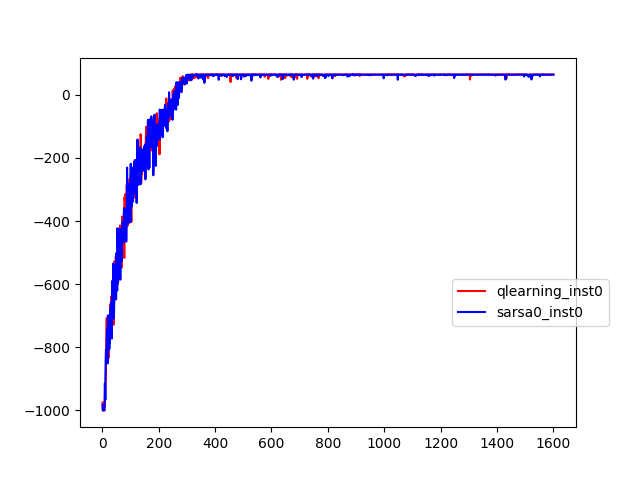
\includegraphics[scale=0.5]{images/qlearn_sarsa0_instance0}
  \caption{Q-learn and Sarsa0 for instance 0}
  \label{fig:ins0}
\end{figure}

\begin{figure}[H]
  \centering
  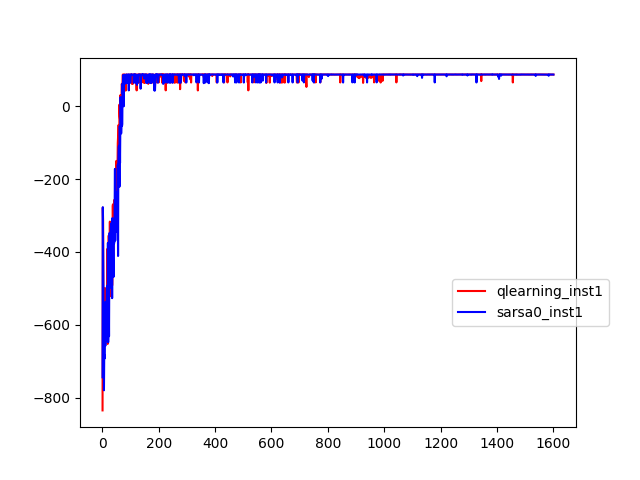
\includegraphics[scale=0.5]{images/qlearn_sarsa0_instance1}
  \caption{Q-learn and Sarsa0 for instance 1}
  \label{fig:ins1}
\end{figure}

\subsection{Plots for Instance 0 and 1 for Q-learning and Sarsa 0.9}
\begin{figure}[H]
  \centering
  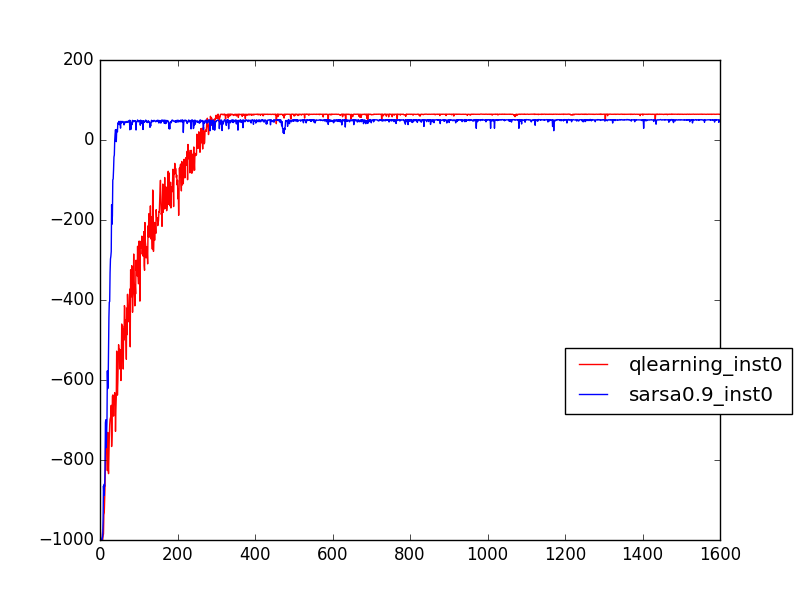
\includegraphics[scale=0.5]{images/qlearn_sarsa0_9_instance_0}
  \caption{Q-learn and Sarsa0.9 for instance 0}
  \label{fig:ins0}
\end{figure}

\begin{figure}[H]
  \centering
  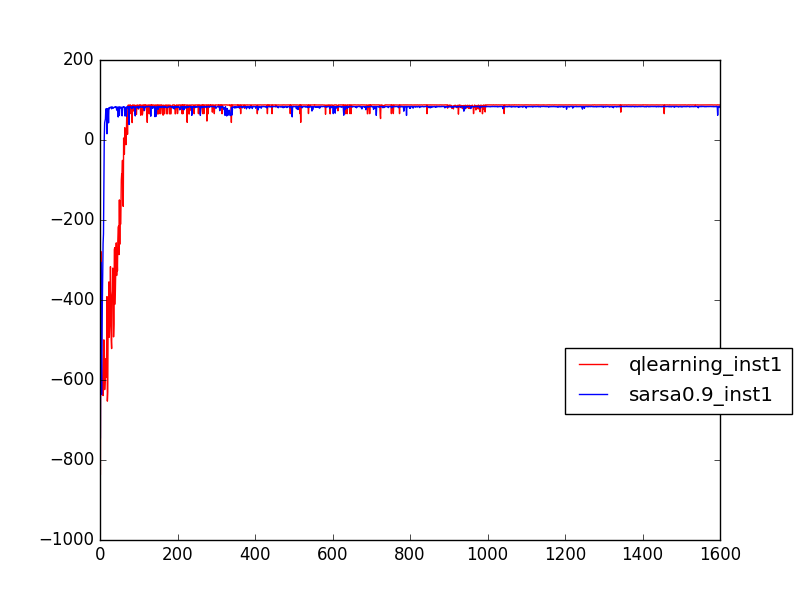
\includegraphics[scale=0.5]{images/qlearn_sarsa0_9_instance_1}
  \caption{Q-learn and Sarsa0.9 for instance 1}
  \label{fig:ins1}
\end{figure}

\subsection{Inference Q-learning vs Sarsa ($\lambda$)}
\begin{itemize}
\item We note that q-learning and sarsa (0) follow almost the same trajectory. Here no annealing of learning rate is done and the same value = 0.5 is used in both cases. Also the epsilon greedy strategy used in both the cases are the same. For q-learning choosing the current action, while for sarsa ($\lambda$) it is the next action.
\item Sarsa(0.9) converges must faster than q-learning but the final convergent value is suboptimal.
\end{itemize}
\section{Expected Cumulative Reward over first 500 episodes vs $\lambda$}
For each value of $\lambda$ we take the expected cumulative reward over first 500 episodes. Here the expectation is over the episodes as well. Therefore we get one value for each value of $\lambda$

\begin{figure}[H]
  \centering
  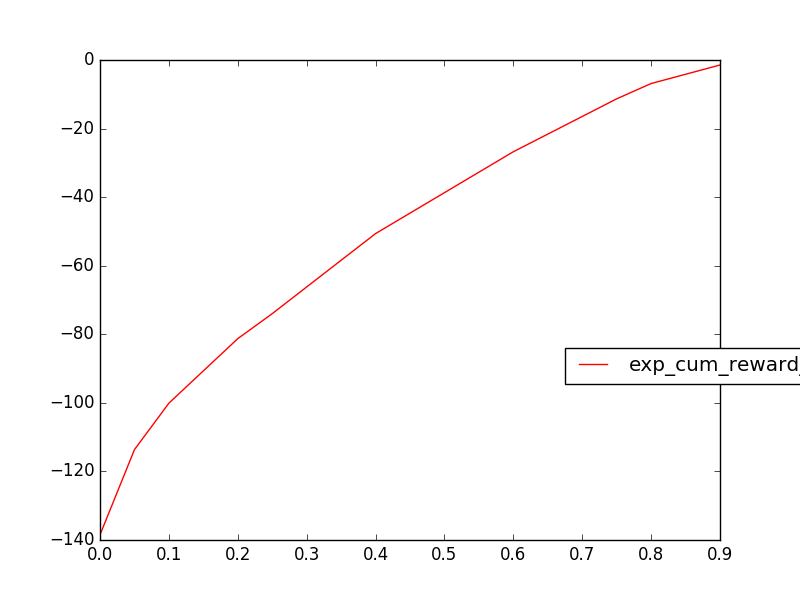
\includegraphics[scale=0.5]{images/sarsa_lamb_instance_0}
  \caption{Sarsa instance 0}
  \label{fig:srsli0}
\end{figure}

\begin{figure}[H]
  \centering
  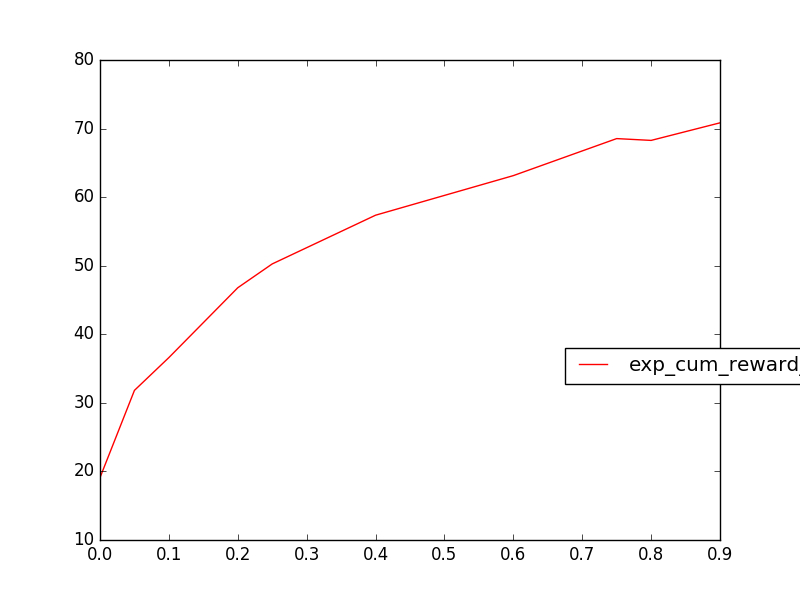
\includegraphics[scale=0.5]{images/sarsa_lamb_instance_1}
  \caption{Sarsa instance 1}
  \label{fig:srsli1}
\end{figure}

In both cases the optimal value is got as 0.9

\subsection{Inference Expected Cumulative reward vs $\lambda$}
\begin{itemize}
\item The $\lambda$ values considered here are :$ [0, 0.05, 0.1, 0.2, 0.25, 0.4, 0.6, 0.75, 0.8, 0.9]$
\item When $\lambda$ is small then the point where it converges is better but it takes more time. When $\lambda$ is larger then it converges faster but to sub-optimal point.
\item Running on $\lambda=1$ results in overflow error, which is because in our case $\gamma=1$ and as a result the eligibility trace blows up because of the large number iteration being done. Therefore it is reasonable to believe the maxima of the curve would be near to $0.9$ and hence this value is chosen.
\end{itemize}

\section{Other Inference and Observations}
\begin{itemize}
\item The most interesting thing was the learning rate parameter. Having a small learning rate lead to much slower convergence, but increasing it lead to faster convergence but occassionally sub-optimal convergent values for some values of $\lambda$ in sarsa.
\item Next is the annealing of $\epsilon$ in $\varepsilon$-greedy method. Aggressive annealing didn't lead to much of a differnce for some reason.
\item Replacing and Accumulation trace gave no difference at all. Doing a diff across two files corresponding to two random seeds gave no difference at all and the trajectory turns out to be exactly identical. Therefore all further experiments related to $\lambda$ tuning were done using accumulative trace.
\end{itemize}


\end{document}